% https://pecorarista.com/posts/poster.html
\documentclass[unicode]{beamer}
\usepackage[orientation=portrait,size=a0,scale=1.7]{beamerposter}
\usetheme[footertext={広葉樹の利用と森林再生についてのワークショップ(東近江市)}]{SimplePoster}

\usepackage{luatexja}
\usepackage{fontspec}
\usepackage{amsmath}
\usepackage{arev}
\setmainfont[Ligatures=TeX]{TeXGyreHeros}
\setsansfont[Ligatures=TeX]{TeXGyreHeros}
\usepackage[dexule,noto-otf]{luatexja-preset}
\renewcommand{\kanjifamilydefault}{\gtdefault}
\renewcommand{\baselinestretch}{1.1}

\usepackage{caption}
\captionsetup[figure]{labelfont={color=black}}

\title{シカが多い地域でのナラ枯れ後の森林の変化}
\author{伊東宏樹}
\institute{森林総合研究所北海道支所}
\date{\today}
\begin{document}
\begin{frame}
\begin{columns}[t]
\begin{column}{.49\linewidth}

\begin{block}{はじめに}
ナラ枯れの被害は依然として続いています。なかには、シカによる影響を受けるものもあります。両方の影響を受けた森林はどのように変化するのでしょうか。

\vspace{2cm}
\centering
\begin{tabular}{cc}
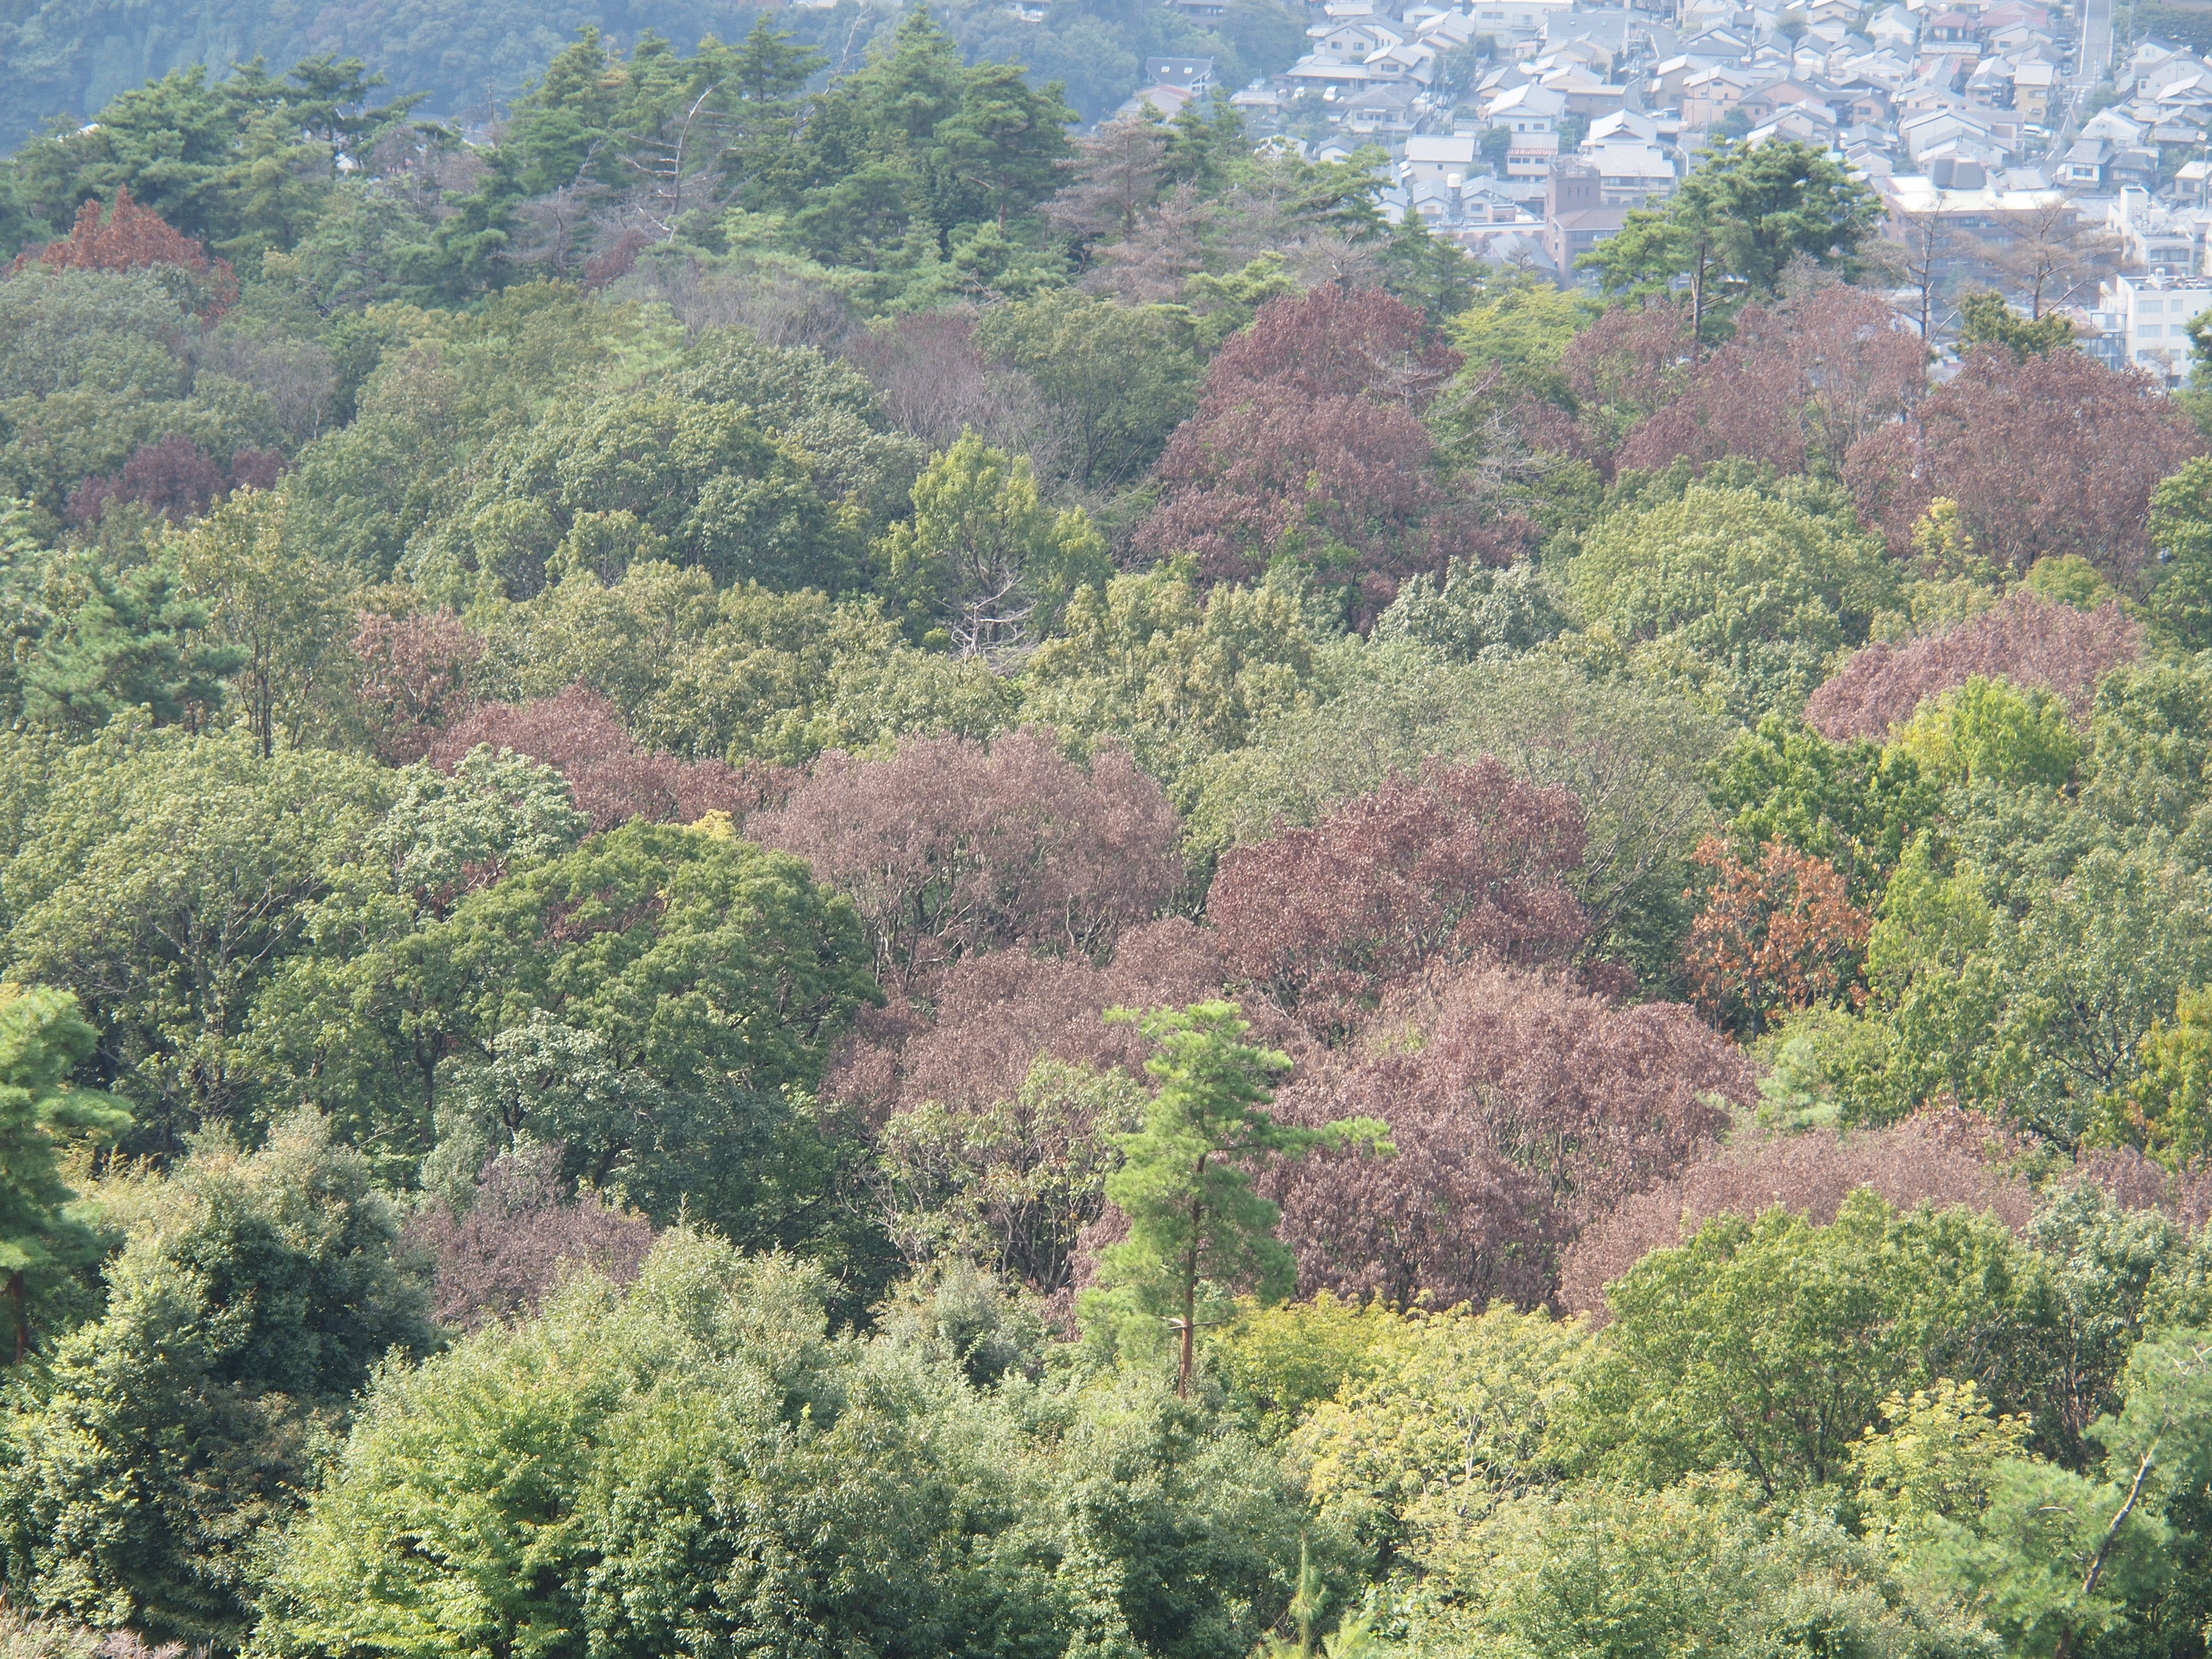
\includegraphics[width=18cm]{photo-2.jpg} &
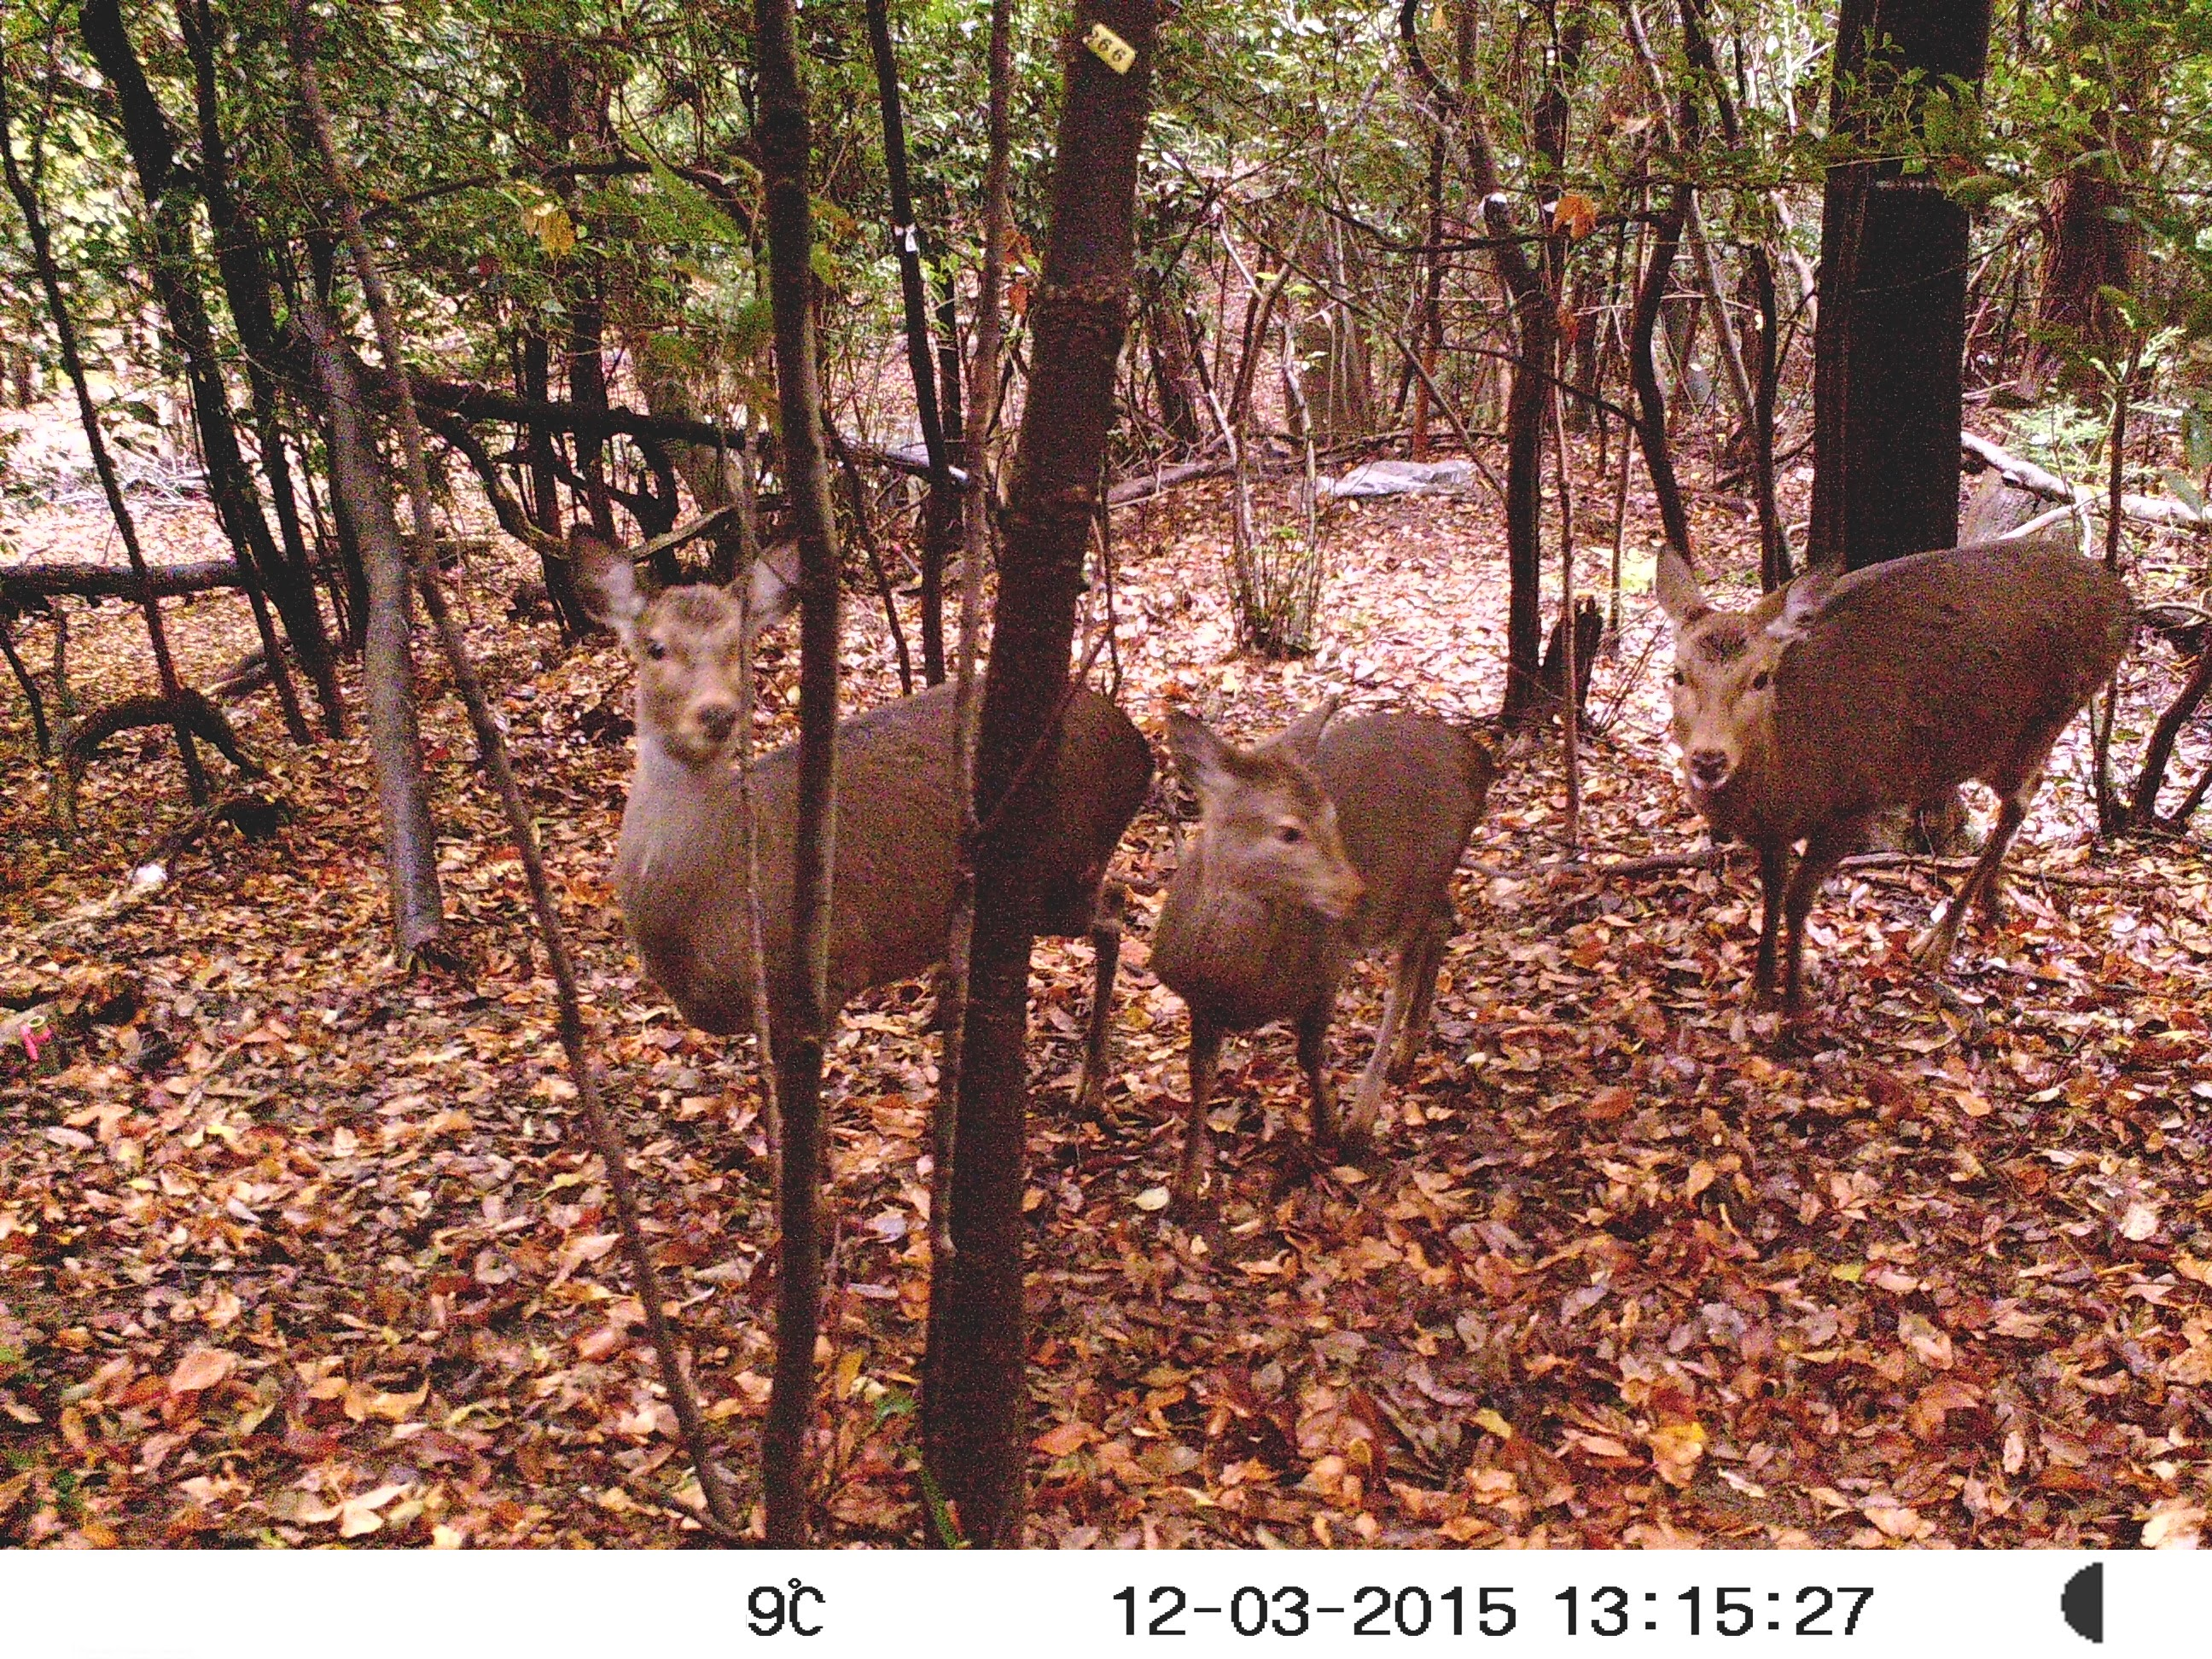
\includegraphics[width=18cm]{photo-3.jpg} \\
{\small ナラ枯れの様子} &
{\small 自動撮影カメラに写ったシカ}
\end{tabular}


\end{block}

\begin{block}{コナラの枯死}
京都東山の銀閣寺山国有林で、0.5haの広葉樹二次林を1993年から継続調査しています。ナラ枯れ発生前の2005年と、後の2014年の胸高断面積合計を比較すると、コナラが大幅に減少したのがわかります。
\vspace{2cm}

%\begin{figure}[htbp]
\centering
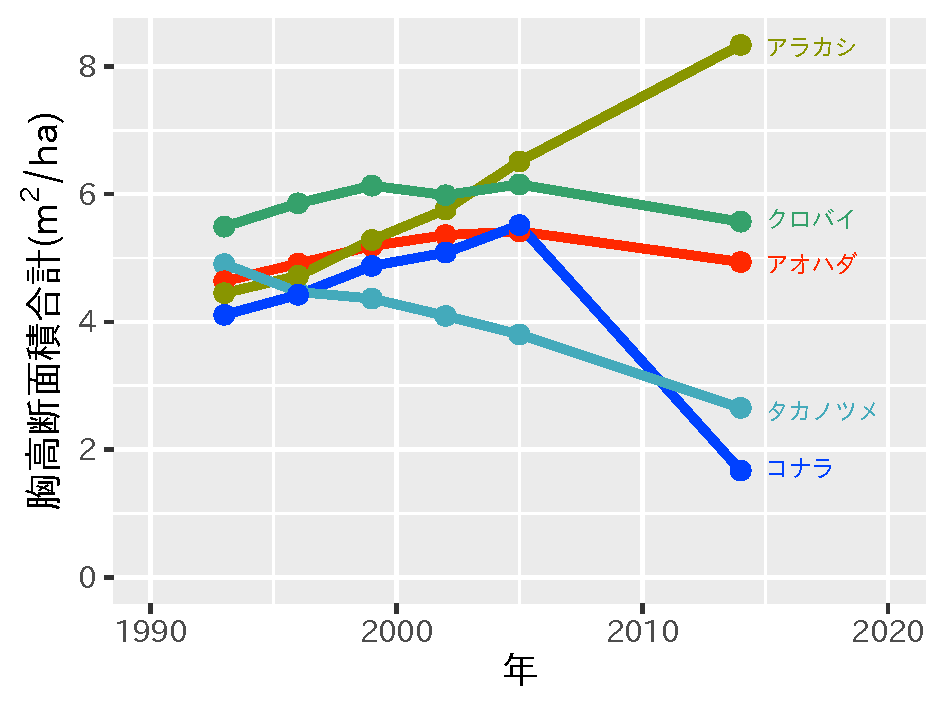
\includegraphics{basal_area.pdf} \\
%\caption{胸高断面積合計の変化}
%\label{fig:ba}\\
{\small 胸高断面積合計の変化}
%\end{figure}
\end{block}


\begin{block}{下層木の変化}
下層木についてみると、全体ではアラカシが依然として高い出現率を維持している一方で、シカが好む低木であるアオキとイヌツゲが激減していました。ナラ枯れによって上層木がなくなったところに限ってみると、クロバイやカラスザンショウ、アカメガシワ、ナンキンハゼといった樹種の出現率が増加していました。このうちクロバイとナンキンハゼはシカが好まない樹種です。

\vspace{2cm}

\centering
\begin{tabular}{cc}
%\begin{figure}[htbp]
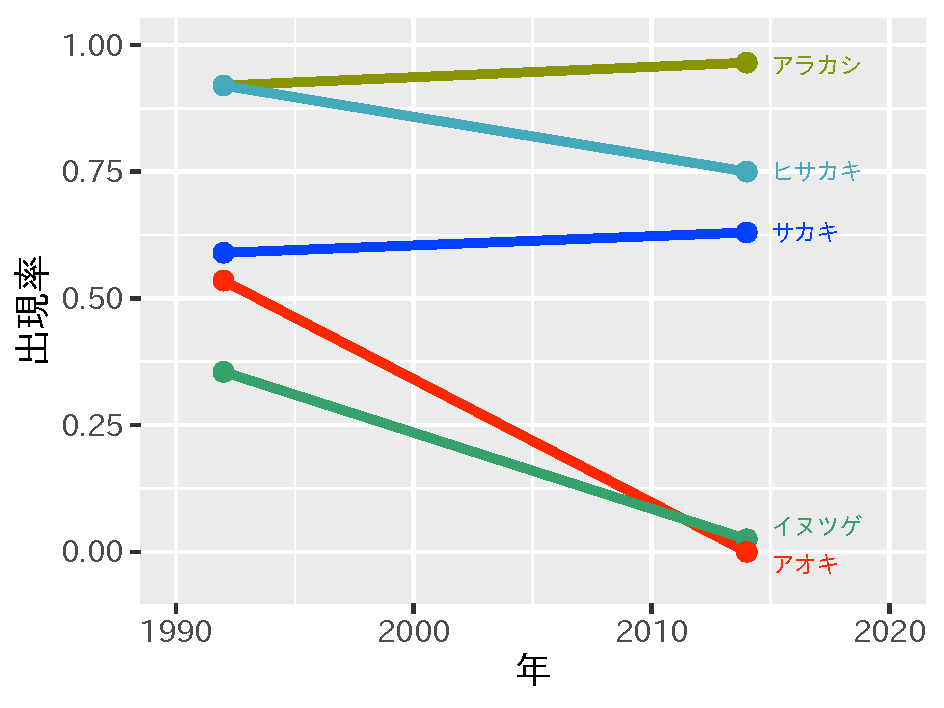
\includegraphics{prop_presense.pdf} &
%\caption{下層木の出現率の変化}
%\label{fig:pro_presense}
%\end{figure}
%\begin{figure}[htbp]
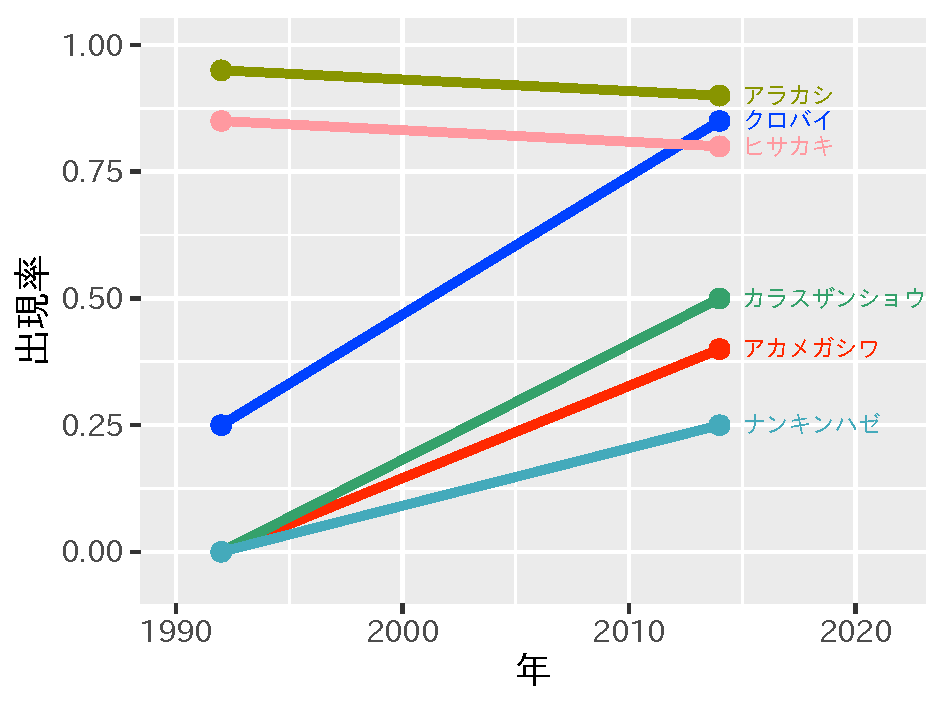
\includegraphics{prop_gap.pdf} \\
%\caption{下層木の出現率の変化(ギャップ内のみ)}
%\label{fig:pro_gap}
%\end{figure}
\multicolumn{2}{c}{\small 下層木の出現率の変化(左:全体, 右:ギャップ内)}
\end{tabular}
\end{block}

\end{column}

\begin{column}{.49\linewidth}
\begin{block}{ギャップに設置したシカ柵の内外での違い}

ナラ枯れによってできたギャップの一部には、京都大阪森林管理事務所がシカ柵を設置しました。
そのシカ柵の内外に、15m×15mの大きさの調査区をそれぞれ設定し、各調査区内で、ナラ枯れ後から3年間の間に新規に1.3m以上にまで成長してきた樹木の樹種と本数を調査しました。その樹高階分布を下の図に示します。

\vspace{3cm}
\begin{tabular}{c}
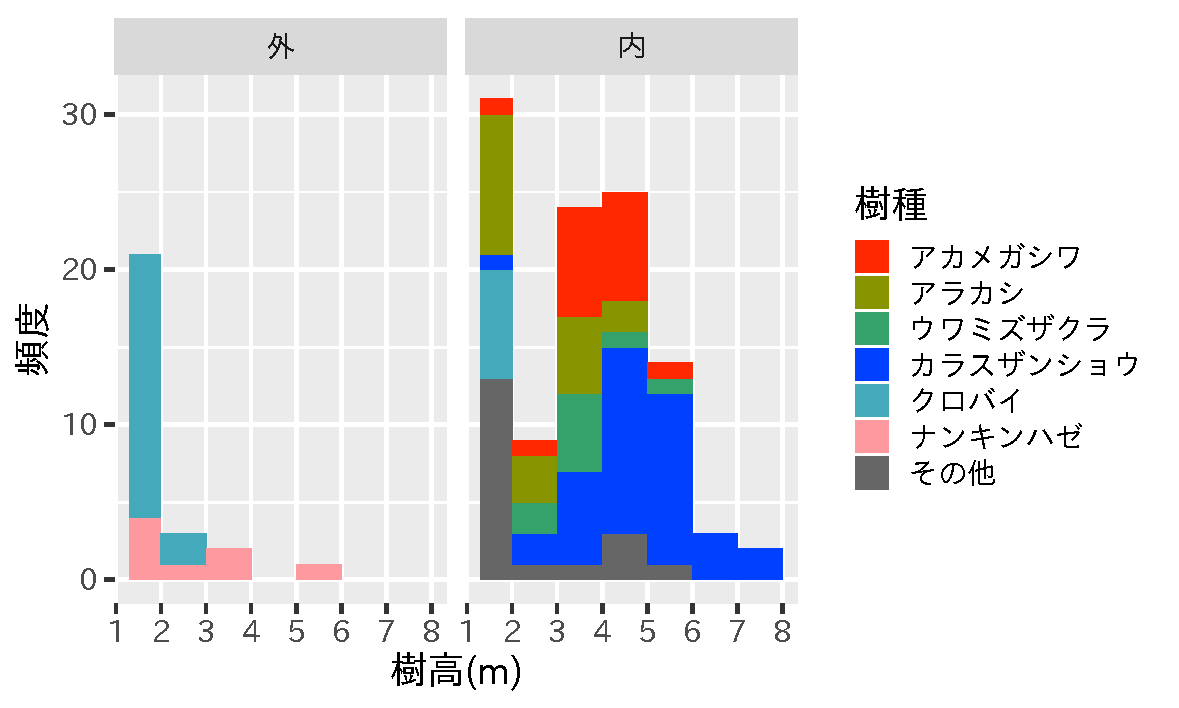
\includegraphics[width=25cm]{fence.pdf} \\
{\small シカ柵内外での更新木の樹高階分布}
\end{tabular}

\vspace{3cm}

シカ柵外(左)では全体として本数が少なく、樹種も、シカが好まないナンキンハゼとクロバイだけだったのに対し、シカ柵内(右)では、本数・樹種とも多く、3m以上にまで成長しているものもかなりあることがわかりました。

{\centering
\vspace{3cm}
\begin{tabular}{cc}
\includegraphics[width=16cm]{IMG_1511.jpg} &
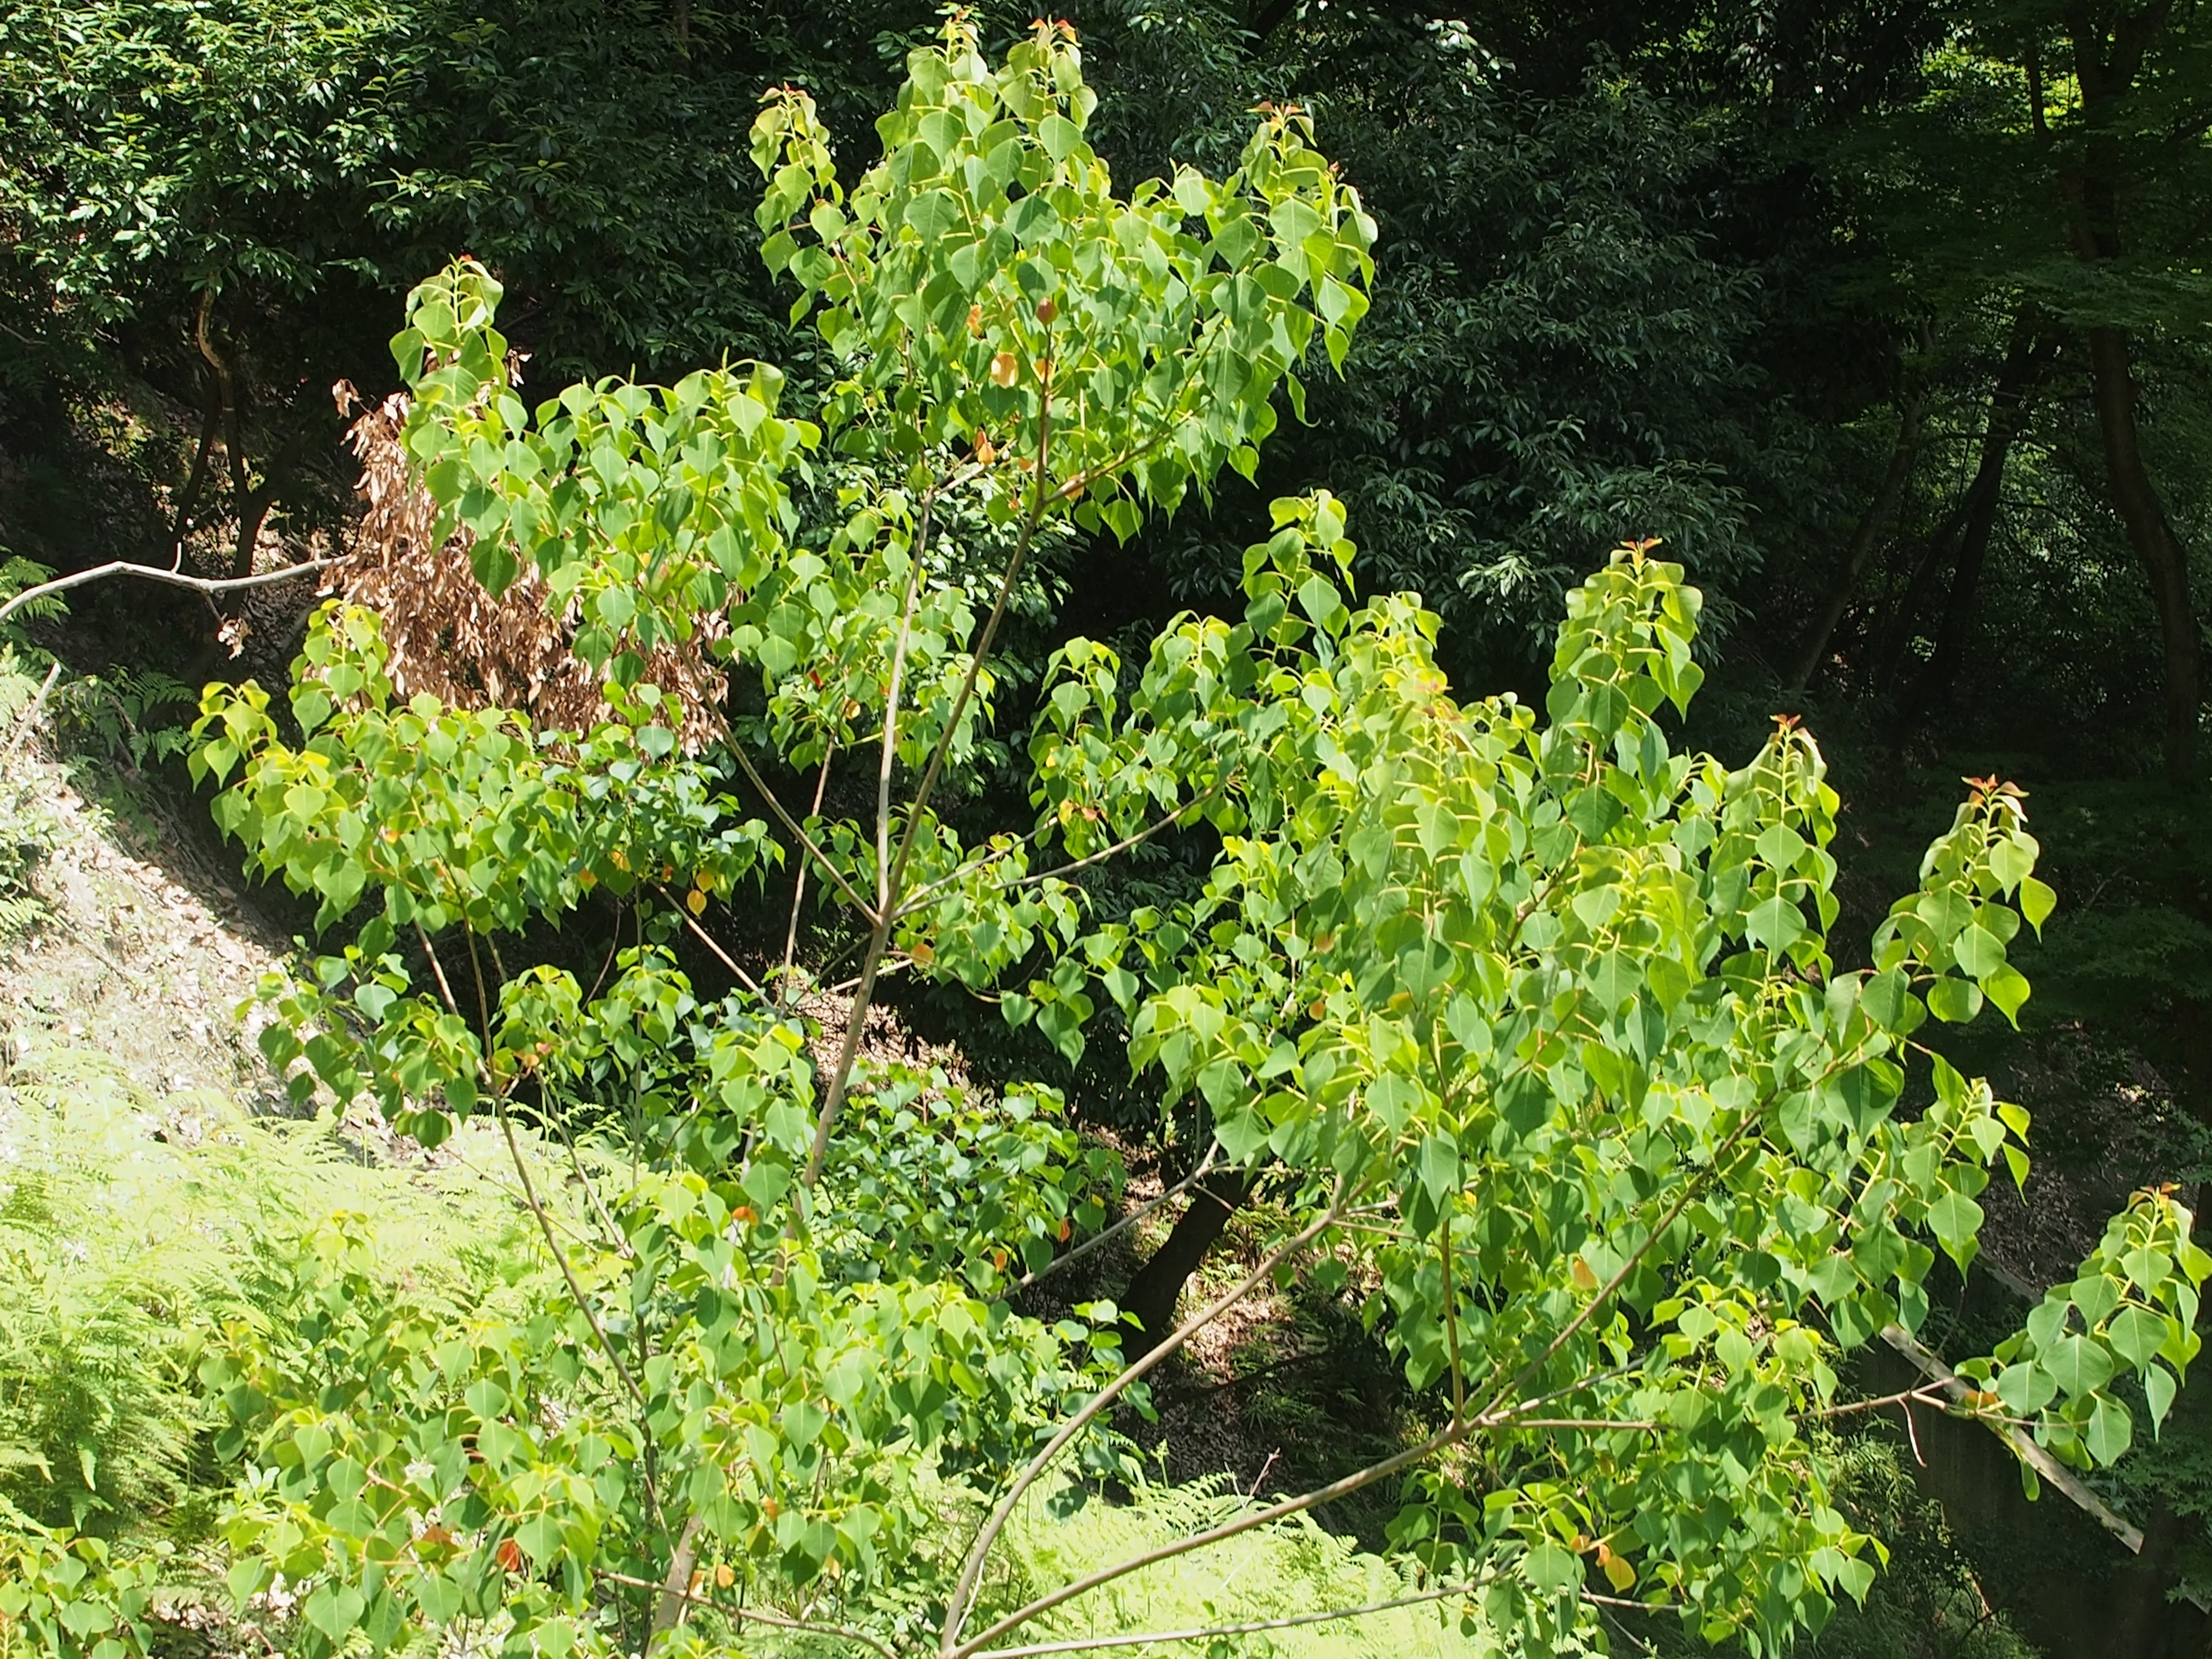
\includegraphics[width=20cm]{photo-4.jpg} \\
{\small シカ柵の内外の状況} &
{\small シカ柵外のナンキンハゼ}
\end{tabular}
}
\end{block}

\begin{block}{まとめ}

シカの多い地域でナラ枯れが発生した場合には、シカが好まない樹種が増加し、シカが少なかったころとは違う森林となる可能性があります。

\vspace{2cm}

しかし、ナラ枯れ発生後にすみやかにシカ柵を設置することで、多様な樹種からなる森林を維持できる可能性があります。

\vspace{2.4cm}

\end{block}

\end{column}
\end{columns}
\end{frame}
\end{document}